\chapter{Visualization}

The super resolution reconstruction process outputs both the reconstructed MRI volume as well as the uncertainty. The uncertainty essentially tells us, for each pixel in the reconstructed volume, how confident are we in that value.

Before the uncertainty can be visualized it is first pre-processed. Firstly the uncertainty is normalized such that values range between 0 and 1, where 0 represents a completely uncertain value is and 1 represents the most certain value in the volume. 

Then there is an optional erosion step which removes the uncertainty values at the edge of the reconstruction. The edges of the reconstruction often have a much higher uncertainty because <put reason here> and if this region isn't of interest for the viewer then removing it helps the visualization to focus on the core of the volume. If, however, the viewer is interested in these areas, then this step can be skipped.

\textbf{MOVE:} As well as the original scans (a.k.a slice stacks) a mask can be provided to ignore areas that are not of interest; for example when doing a fetal brain scan a mask is created to ignore surrounding areas like the womb and amniotic fluid.

% Idea -> Implementation -> Results
\section{Thresholding}\label{section:thresholding}

The idea behind thresholding is to isolate areas in the reconstructed image within a particular range of uncertainty. This allows the viewer to highlight regions in a specified range (e.g. 0.2 to 0.5) and also lets them isolate the worst values in the volume (e.g. the worst 1$\%$).

\subsection*{Implementation}
The implementation uses a filter provided by ITK to go create a binary mask which is set to 1 where the uncertainty is in the range and 0 where it is not. This mask is then overlayed on the reconstructed scan in 2D and made transparent so both the uncertain area and underlying scan can be seen simultaneously.

This thresholded mask is also displayed in 3D using volume rendering (see section \ref{background:volumerendering}). In this case the transfer function maps a value of 0 (out of the range) to be completely transparent and a value of 1 (in the range) to be opaque.

\begin{figure}
  \centering
  \begin{subfigure}[b]{0.5\textwidth}
    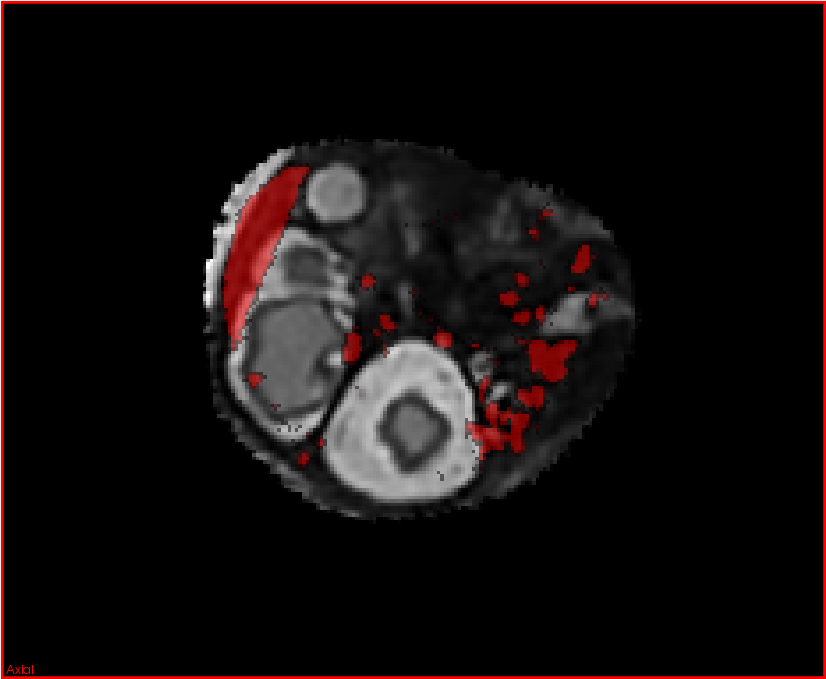
\includegraphics[width=\textwidth]{images/thresholding_2d.png}
    \caption{2D Thresholding}
    \label{fig:thresholding2d}
  \end{subfigure}%
  ~ %add desired spacing between images, e. g. ~, \quad, \qquad, \hfill etc.
    %(or a blank line to force the subfigure onto a new line)
  \begin{subfigure}[b]{0.5\textwidth}
    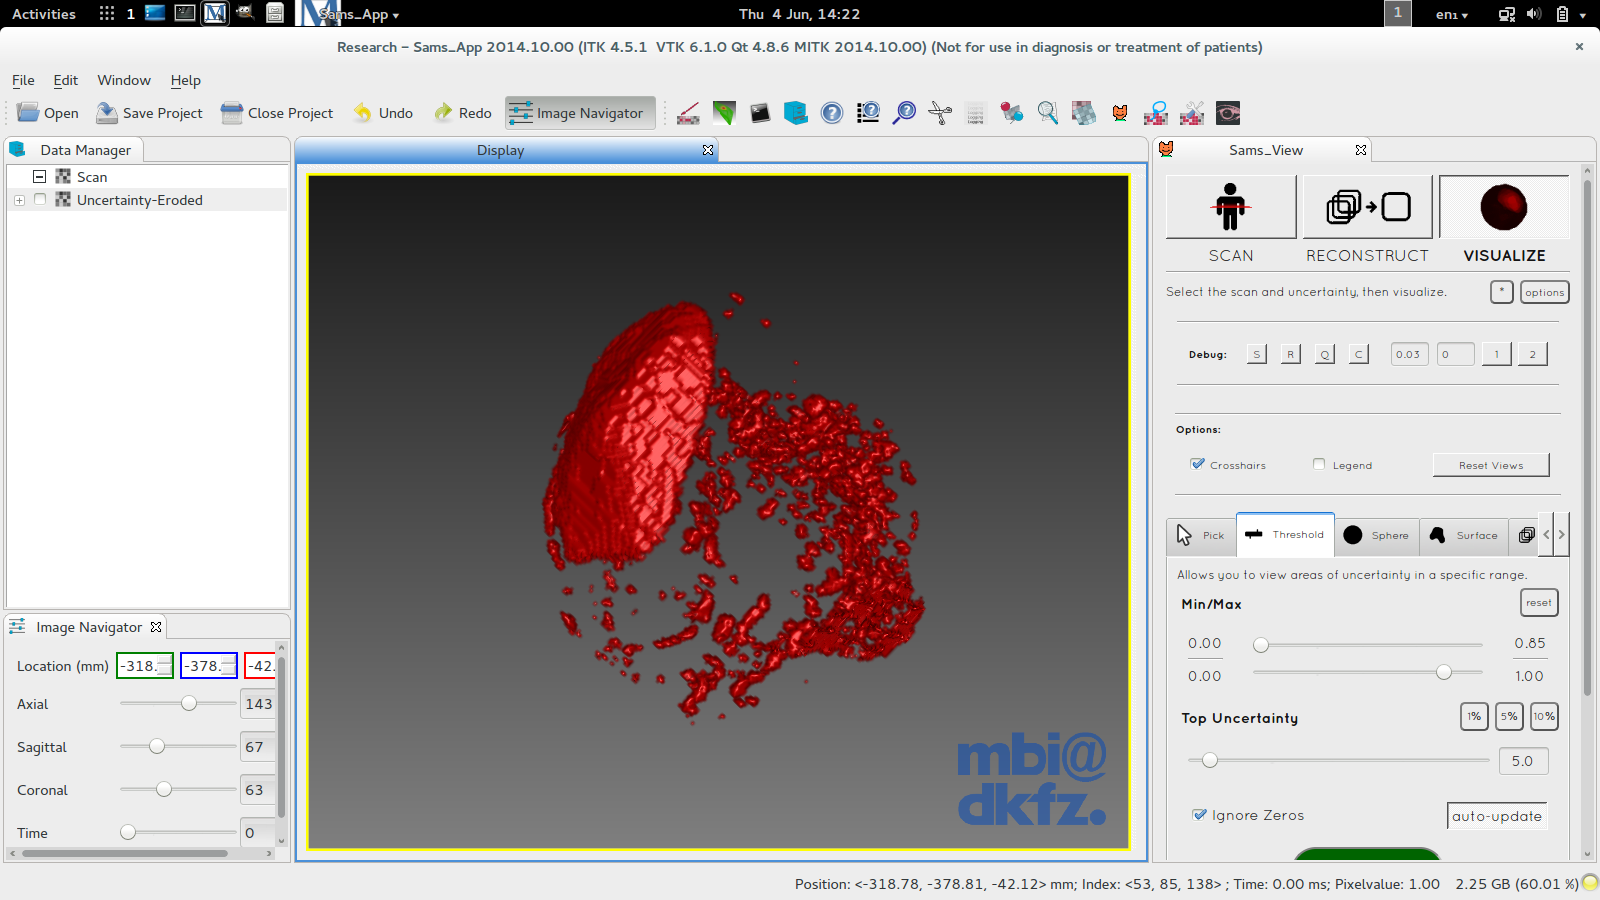
\includegraphics[width=\textwidth]{images/thresholding_3d.png}
    \caption{3D Thresholding}
    \label{fig:thresholding3d}
  \end{subfigure}
  \caption{Example showing the worst 5$\%$ of an example reconstruction.}\label{fig:threshldingoverview}
\end{figure}

\subsection*{Results}
// Compare with applying transfer function to actual uncertainty. Illustrate the problems with small dots.


\section{Uncertainty Surface}\label{section:uncertaintysurface}

\section{Next Scan Plane}\label{section:nextscanplane}

\chapter{Tool}

\section{Scan Simulation}\label{section:simulatescan}

\section{Reconstruction}\label{section:reconstruction}